

\section{引言}
粒子群优化算法(Particle Swarm Optimization, PSO)属于计算智能领域,是由美国社会心理学博士Kennedy和电气工学博士Eberhart于1995年提出的一种全局搜索算法。该算法源于对鸟群觅食过程中的迁徙和群居行为的模拟,是一种模拟自然界的生物活动以及群体智能的随机搜索算法。群体中的每个粒子位置代表搜索空间中的一个候选解。粒子个体之间通过位置信息的交流和学习来调整各自搜索方向。粒子群优化由于其算法简单,易于实现,无需梯度信息,参数少等特点在连续优化问题和离散优化问题中都表现出良好的效果,特别是因为其天然实数编码特点适合于处理实优化问题,近年来成为国际上智能优化领域研究的热门。作为一种重要的优化工具,粒子群优化算法已经成功地用于目标函数优化,神经网络训练,模糊控制系统,模式识别,信号处理,图形图像处理,统计学习模型参数优化,机器学习模型参数优化等领域。
%\cite{Figueredo:2009dg}.

%\begin{table}[hbt]
%	\caption{这是一张无聊的表}
%	\centering
%	\begin{tabular}{llr}
%		\toprule
%		\multicolumn{2}{c}{姓名} \\
%		\cmidrule(r){1-2}
%		名名名名名名 & 姓姓姓姓姓姓 & 分数 \\
%		\midrule
%		雷 & 张 &~$7.5$~\\
%		梅梅 & 王 &~$2$~\\
%		\bottomrule
%	\end{tabular}
%	\label{tab:label}
%\end{table}
\subsection{粒子群算法的发展}
PSO模拟鸟群随机搜索食物的捕食行为。假设在搜索食物区域里只有一块食物,所有的小鸟都不知道食物在什么地方,所以Kenndy等认为鸟之间存在信息的相互交换,通过估计自身的适应度值,得到离食物的距离。所以鸟群通过集体协作寻找最优解,搜索离食物最近的鸟的周围区域是一种有效方法。PSO算法将每个潜在解想象成搜索空间中的一只鸟,称为“粒子”。粒子重要追随当前最优粒子在解空间中搜索。

PSO首先初始化一群随机粒子,作为初始种群,然后通过不断地迭代寻优寻找最优解。在每一次迭代中,粒子通过跟踪两个“极值”来更新自己,第一个是粒子本身在历代迭代中寻找到的最优解,称为个体极值pBest,另一个极值是整个种群自迭代之初到目前所寻找到的最优解,称为全局极值gBest。这两个最优变量指引粒子们的运动。此外,全局极值也可由局部极值代替,即某几个粒子组成一个邻域,彼此之间共享信息引导邻域粒子的运动。粒子始终跟随两个极值,每次迭代中更新自己的速度和位置,直到找到最优解。

与其他优化算法一样,粒子群算法也存在“过早收敛”的问题。过早收敛又称为“早熟”(Premature Convergence),是指当前算法在搜索演化过程中,迭代到一定程度后陷入到一种非全局最优状态。同时,粒子群算法并不能从理论上严格证明其收敛于任何类型函数的全局最值点。Vanden Bergh证明了传统标准PSO算法虽然高效,但并不能保证一定收敛于全局最优点,也不能保证搜索不到全局最优点,而是以一定概率搜索到全局最优。到目前为止,粒子群算法的发展得到越来越多领域及其学者的关注和研究,算法被不断应用于各种优化问题的求解。针对PSO算法存在的问题,国内外学者主要从以下四方面对算法进行改进:参数的调整、种群拓扑结构的改变、算法融合、小生境技术。

目前,粒子群算法的发展趋势如下:


	\noindent (1) 粒子群优化算法的改进。粒子群优化算法在解决连续问题和单目标问题中应用较多,如何使其应用于离散问题和多目标问题是PSO算法的重要研究方向。如何充分结合其他进化类算法,发挥优势,改进PSO算法的不足也是值得研究的。
	
	\noindent (2) 粒子群优化算法的理论分析。PSO算法提出时间不长,数学基础薄弱,对算法的运行行为、收敛性、计算复杂性的研究不足。如何指导参数的选择和设计、如何设计适应值函数、如何提高算法效率及保证收敛都是PSO算法的研究方向。
	
	\noindent (3) 粒子群算法的生物学基础。如何根据群体行为完善算法、将群体智能注入算法中,借鉴生物群体进化规则和进化的智能性也是研究方向之一。
	
	\noindent (4) 粒子群优化算法与其他进化类算法的比较研究。与其他进化算法的融合,如何将其他进化算法的优点与粒子群算法相结合,构造出有特色有使用价值的混合算法是当前算法改进的一个重要方向。
	
	\noindent (5) 粒子群优化算法的应用。算法的有效性必须在应用中才能体现。广泛地开拓粒子群算法的应用领域,对深入研究粒子群算法具有指导意义。

	
\subsection{粒子群算法研究内容}
粒子群算法是非常简单的算法,能够有效地优化各种函数。从某种程度上来说,此算法介于遗传算法和进化规划之间。PSO算法非常依赖随机过程,这也是和进化规划的相似之处。算法中朝全局最优和局部最优靠近的调整类似于遗传算法中的交叉算子。

\noindent 粒子群算法的主要研究内容如下:

(1)	寻找全局最优点。

(2)	有较高的收敛速度。

算法还使用了适应值的概念,这是所有进化算法所共有的特征。

\subsection{粒子群算法的特点}
粒子群算法本质是一种随机搜索算法,它是一种新兴的智能优化技术,是群体智能中一个分支,也是对简单社会系统的模拟。该算法较传统优化算法具有更快的速度和更好的全局搜索能力。其特点如下:
\begin{itemize}
	\item 粒子群优化算法是基于群体智能理论的优化算法,是通过群体粒子间的合作与竞争产生的群体智能指导优化搜索。与进化算法比较,PSO是一种更高效的并行搜索算法。
	
	\item PSO与GA有很多共同之处,两者都是随机初始化种群,使用适应值来评价个体优劣程度,再进行随机化搜索。但PSO采用了速度-位移模型,操作简单,避免复杂的遗传操作,且保留了基于种群的全局搜索策略。
	
	\item 每个粒子在算法结束时仍保留个体极值,因此,若将PSO用于调度和决策问题时可以给出多种有意义的选择方案。
	
	\item PSO特有的记忆使其可以动态地跟踪当前搜索情况并调整其搜索策略。
	
	\item PSO算法本身的特征,使其在搜索过程中能较好得保持多样性和方向性。
	
	\item 在收敛的情况下,迭代后期粒子趋向同一化,收敛速度明显变慢,收敛到一定精度时便无法继续优化。
	
	\item PSO算法对种群规模不敏感,即使种群数目下降,对算法的性能影响也不大。
\end{itemize}
	

\subsection{粒子群算法的应用}
粒子群算法提供了一种求解优化问题的通用框架,对问题具有很强的适应性,广泛应用于各种学科。其应用的意义在于:在给定的条件下寻找到最好的解决方案,使得资源发挥出最大效用。其重要应用领域如下:
\begin{itemize}
	\item 工程设计与优化领域。神经网络训练、RBF网络优化、控制器设计与优化、电路及滤波器设计优化。
	\item 电力系统领域。最优潮流计算、电网扩展计划、电力恢复系统、检修计划、机组优化组合、电容器优化配置。
	\item 交通运输领域。车辆路径优化问题、物流VRP配送问题、交通控制优化问题、机器人路径规划问题。
	\item 计算机领域。数据挖掘分类问题、图像处理、任务分配。
	\item 信息通信领域。路由选择及以移动通信基站布置优化、天线阵列控制优化、偏振模色散控制优化。
\end{itemize}
 

\subsection{本文研究内容}
本文主要就传统粒子群算法的产生、研究现状及算法原理进行解释,同时列举出多种粒子群算法的改进版本,进行解释与分析比较,最后将标准粒子群算法与其改进算法进行仿真实验,对比研究,得出结论。
\section{粒子群算法原理}
粒子群优化算法是建立在群体智能基础上的随机演化方法。算法通过模拟自然界鸟类捕食行为来进行问题解空间的探索,并根据个体对环境的适应度(Fitness Value)移动位置。鸟群通过各自的探索和群体的合作最终发现食物所在位置。各个鸟在飞行过程中不断地记录和更新它曾经到达的离食物最近的距离,同时,它们通过信息交流的方式比较大家所找到的最好位置,得到一个当前整个群体已经找到的最佳位置。这样,每个小鸟在飞行的时候就有了一个指导的方向,它们会结合自身的经验和整个群体的经验,调整自己的飞行速度和所在位置,不断地寻找更加接近食物的位置,最终使得群体聚集到食物位置。

\subsection{基本粒子群优化算法}
PSO算法起源于对简单社会系统的模拟,具有很好的生物社会背景,在科学研究与工程实践中得到了广泛的关注。其易理解、参数少易实现、对线性、多峰问题具有较强的全局搜索能力的特点使其成为一种很好的优化工具。
\subsubsection{算法原理}
基本粒子群优化算法是粒子群算法的初始版本。一个由m个粒子(Particle)组成的群体(Swarm)在D维搜索空间中以一定的速度飞行,每个粒子在搜索时,考虑到了自己搜索到的历史最好点和群体内(或邻域内)其他粒子的历史最好点,在此基础上进行位置的变化。

 \noindent 第i个粒子的位置表示为:
 
 \centerline{$x_i=[x_i^1,x_i^2,x_i^3,$……$,x_i^D]$}


 \noindent 第i个粒子的速度表示为:
 
 \centerline{$v_i=(v_i^1,v_i^2,v_i^3,$……$,v_i^D),1\leq i\leq m$} 

\noindent 第i个粒子经过的历史最好点表示为:$p_{Best}$

 群体内(或邻域内)所有粒子经过的最好点表示为gBest,这个全局最优向量起到引导粒子向该全局最优区域收敛的作用。

一般来说,粒子的位置和速度都是在连续的实数空间内进行取值。
\subsubsection{算法流程}

基本粒子群优化算法流程如下:
\begin{enumerate}
	\item 初始化所有粒子,对粒子的位置和速度进行随机初始化,并将个体的历史最优pBest设为当前位置,群体中最优个体作为当前gBest。
	\item 计算各个粒子的适应度函数值。
	\item 对每个粒子,将其历史最优适应值于群体内所经历的最好位置的适应值进行比较,若更好,则将其作为当前全局最好位置。
	\item 对每个粒子,将其历史最优适应值与所经历过的最好位置的适应值进行比较,若果更好,则将其作为当前全局最好位置。
	\item 对每个粒子i的第d维速度和位置分别按照公式(\ref{BPSO})和公式(\ref{location})进行更新。
	\begin{equation}
	\begin{split}
	\label{BPSO}
	v_i^d=v_i^d+&c_1*{rand}_1^d*({pBest}_i^d-x_i^d )+\\
	&c_2*{rand}_2^d*({gBest}^d-x_i^d)
	\end{split}
	\end{equation}
	\begin{equation}
	\label{location}
	x_i^d=x_i^d+v_i^d
	\end{equation}
	
	\item 若未达到终止条件,则转第二步。一般将终止条件设定为一个足够好的适应值或达到一个预设的最大迭代代数。
\end{enumerate}

其中,c1和c2称为学习因子(Learning Factor)或加速系数(Acceleration Coefficient), 学习因子使粒子具有自我总结和向群体中优秀个体学习的能力,从而向自己的历史最优点以及群体内的历史最优点靠近,传统上都是取固定值2.0。${rand}_1^d$和${rand}_2^d$是两个[0,1]区间上的随机数。粒子速度被限制在最大速度$V_{max}$内,$V_{max}$的每一维$V_{max}^d$一般可以取相应维的取值范围的10\%—20\%。另外公式(\ref{location})中的位置更新必须是合法的,所以在每次进行更新之后必须进行合法性检测,对越界的位置,需要进行合法性调整,一般的修正方法可以是重新随机设定或限定在边界。

\subsubsection{粒子的社会行为分析}
从粒子速度更新方程\ref{BPSO}可以看到,基本粒子群优化算法中,粒子的速度主要由三部分构成。
\begin{enumerate}
	\item \textbf{前次迭代中自身的速度}
	\noindent 式(\ref{BPSO})右侧第一项,这是粒子飞行中的惯性作用,是粒子能够进行飞行的基本保证。
	
	\item \textbf{自我认知的部分}
	\noindent 式(\ref{BPSO})右侧第二项,表示粒子飞行中考虑到的自身的经验,向自己曾经找到过的最好点靠近。
	
	\item \textbf{社会经验的部分}
	\noindent 式(\ref{BPSO})右侧第三项,表示粒子飞行中考虑到社会的经验,向邻域中其他粒子学习,使粒子在飞行时向全局最好点靠近。
\end{enumerate}
\subsection{标准粒子群优化算法(Standard PSO Algorithm)}
为改善算法收敛性能,Shi和Eberhart在1998年的论文中进入了惯性权重的概念。惯性权重算法的位置更新公式沿用基本PSO中的位置更新公式(\ref{location}),速度更新公式如下(\ref{PSOV})所示,
\begin{equation}
\begin{split}
\label{PSOV}
v_i^d=\omega\times v_i^d+&c_1*{rand}_1^d*({pBest}_i^d-x_i^d)+\\ &c_2*{rand}_2^d*({gBest}^d-x_i^d)
\end{split}
\end{equation}

在Shi和Ebhert的研究中,惯性权重以线性递减的方式从0.9降为0.4,权重在调节过程中,粒子搜索的情况也逐渐由基于全局的广度搜索逐步过渡到基于局部深度搜索,实现了全局搜索和局部搜索的平衡,减弱甚至消除基本粒子群算法中因速度最大数值边界处理时对算法性能的影响。比较好的优化策略是在前期,算法具备比较好的广度搜索能力,以便得到优秀的种子解,后期搜索算法应具有较好的深度搜索能力,以便加快算法的收敛速度。

惯性权重ω体现了当前粒子继承上一代粒子速度的能力。当$\omega$=1时,算法退化成为基本粒子群算法;当$\omega$$\ge$1时,粒子速度随迭代次数的进行而逐渐增加,容易使粒子飞过最优解;当0$\le$$\omega$$\le$1时,粒子在演化过程中速度逐渐降低,收敛性能此时取决于加速参数c1和c2。

目前,对粒子群优化算法的研究大多以带有惯性权重的粒子群优化算法为对象进行分析、扩展和修正,因此大多数文献中将带有惯性权重的粒子群优化算法称为粒子群优化算法的标准版本,或者称为标准粒子群优化算法;而将前述粒子群优化算法称为初始粒子群优化算法/基本粒子群优化算法。

\subsection{算法构成要素}
基本粒子群算法构成要素包括粒子群编码方法、个体适应度评价和基本粒子群算法运行参数三个部分。这里对粒子群优化算法构成要素进行概述。其中粒子群算法运行参数包括算法的相关参数:群体大小、学习因子、最大速度、惯性权重。也包括邻域拓扑结构、粒子空间的初始化和停止准则。
\subsubsection{粒子群编码方法}
基本粒子群算法使用固定长度的二进制符号串来表示群体中的个体,其等位基因是由二值符号集{0,1}所组成的。初始群体中各个个体的基因值可用均匀分布的随机数来生成。
\subsubsection{个体适应度评价}
通过确定局部最优迭代达到全局最优收敛,得出结果。
\subsubsection{基本粒子群算法的运行参数}
\begin{enumerate}
	\item \textbf{群体大小m}
	\noindent m是整型参数。当m很小时,陷入局优的可能性很大;当m很大时,会导致计算时间大幅增加,收敛速度非常慢。
	\item \textbf{学习因子c1和c2}
	\noindent 学习因子使粒子具有自我总结和向群体中优秀个体学习的能力,从而向群体内或邻域内最优点靠近。C1和c2通常等于2,不过也有其他取值。但是一般c1等于c2,并且范围在0和4之间。
	\item \textbf{最大速度$V_{max}$}
	\noindent 最大速度决定粒子在依次迭代中最大的移动距离。$V_{max}$较大时,探索能力强,但容易飞过最好解;$V_{max}$较小时,开发能力强,但容易陷入局优。有分析和实验表明,$V_{max}$的作用可以通过惯性权重$\omega$的调整来实现,故现在实验基本上使用$V_{max}$进行初始化。
	\item \textbf{惯性权重$\omega$}
	\noindent 智能优化方法的运行是否成功,探索能力和开发能力的平衡是非常关键的。对粒子群优化算法来说,这两种能力的平衡是靠惯性权重来实现的。当$\omega$较大时,粒子具有更好的探索能力;当$\omega$较小时,粒子具有更好的开发能力。
	\item \textbf{邻域拓扑结构}
	\noindent 全局版本粒子群优化算法将整个群体作为邻域,速度快,不过有陷入局优的可能性;局部版本粒子群优化算法将索引号相近或位置相近的个体作为粒子的邻域,收敛速度慢,但不易陷入局优。
	\item \textbf{停止准则}
	\noindent 一般使用最大迭代次数或可以接受的满意解作为停止准则。
	\item \textbf{粒子空间的初始化}
	\noindent 较好地选择粒子的初始化空间,将大大缩短收敛时间。这是问题依赖的。
\end{enumerate}
\section{PSO的改进与变形}
这一节,首先介绍算法的三个构成要素的选择和调节:惯性权重、邻域拓扑结构和学习因子;然后介绍粒子群优化算法另一个重要的改进版本:带有收缩因子的粒子群优化算法;再针对离散优化问题,说明两个典型的离散版本粒子群优化算法;之后,介绍几种基于遗传思想和梯度信息的改进策略;最后是算法在两类复杂环境中的解决方案:约束优化和多目标优化。
\subsection{三个构成要素的选择和调节}
\subsubsection{惯性权重}
惯性权重是标准粒子群优化算法的重要参数,对算法的好坏起着决定性作用。Nickabadi等人将不同的惯性权重划分为三种类型:1.常数权重和随机权重,如$\omega$=0.721或$\omega$=0.5+rand()/2.0
	2.基于时间的动态权重,如$\omega={(\frac{2}{iter})}^{0.3}$或$\omega=(\frac{{iter}_{max}-{iter}_i}{{iter}_{max}})*(\omega_{init}-\omega_{end})+\omega_{end}$3.自适应权重,这类权重的设置通常建立在反馈的机制上。
\begin{enumerate}
	\item \textbf{固定权重}
	
	\hspace{2em} 即赋予惯性权重以一个常数值,一般来说,该值在0和1之间。固定的惯性权重使粒子在飞行中始终具有相同的探索和开发能力。显然,对于不同的问题,获得最好优化效果的这个常数是不同的,通常需要大量的实验来确定该常数值。通过实验发现,种群规模越小,需要的惯性权重越大,因为此时种群需要更好的探索能力来弥补粒子数量的不足,否则粒子极易收敛;种群规模越大,需要的惯性权重越小,因为每个例子可以更专注于搜索自己附近的区域。
	\item \textbf{随机权重}
	
	\hspace{2em}随机权重是在一定范围内随机取值。例如可以取值如下$$\omega=0.5+\frac{Random}{2}$$
	
	其中Random为0—1之间的随机数。这样,惯性权重将在0.5—1之间随机变化,均值为0.75.之所以这样设定,是为了应用于动态优化问题。将惯性权重设定为线性减小的时变权重是为了在静态的优化问题中使粒子群在迭代开始的时候具有较好的全局搜索能力,在迭代后期具有较好的局部搜索能力。而对于动态优化问题来说,不能预测在给定的时间粒子群需要更好的全局搜索能力还是局部搜索能力,所以可以使惯性权重在一定范围内随机变化。
	\item \textbf{时变权重}
	
	\hspace{2em}一般来说,希望粒子群在飞行开始的时候具有较好的探索能力,而随着迭代次数的增加,特别是在飞行的后期,希望具有较好的开发能力。可以通过时变权重的设置来实现。Shi.Y提出了线性递减惯性权重(Linear Decreasing Intertia Weight,LDIW),即$$\omega(k)=\frac{\omega_{start}*(\omega_{start}-\omega_{end})*(T_{max}-k)}{T_{max}}$$
	
	\hspace{2em}其中,$\omega_{start}$为初始惯性权重;$\omega_{end}$为迭代至最大次数时的惯性权重;k为当前迭代代数;$T_{max}$为最大迭代代数。一般来说,惯性权值$\omega_{start}$=0.9,$\omega_{end}$=0.4时算法性能最好。这样,随着迭代的进行,惯性权重由0.9线性递减至0.4,记带有线性递减惯性权重的粒子群优化算法为LDIW-PSO。迭代初期较大的惯性权重使算法保持了较强的全局搜索能力,而迭代后期较小的惯性权重有利于算法进行更精确的局部搜索。这是一种线性减小的变化方式,也可以采用非线性减小的变化方式来设置惯性权重。
	
	\hspace{2em}常用的惯性权重的选择还包括如下几种:$$\omega(k)=\omega_{start}-(\omega_{start}-\omega_{end})(\frac{k}{T_{max}})^2$$
	$$\omega(k)=\omega_{start}+(\omega_{start}-\omega_{end})[\frac{2k}{T_{max}}-(\frac{k}{T_{max}})^2]$$
	$$\omega(k)=\omega_{end}(\frac{\omega_{start}}{\omega_{end}})^{\frac{1}{1+\frac{ck}{T_{max}}}}$$
	$$\omega(k)=\omega_{max}-k*\frac{\omega_{max}-\omega_{min}}{T_{max}}$$
	
	\hspace{2em}根据实际问题来确定最大权重$\omega_{max}$和最小权重$\omega_{min}$。线性时变权重是在实际应用中使用最为广泛的一种方式。
	\item \textbf{自适应权重}
	
	\hspace{2em}这种类型的权重一般需要对群体的搜索情况的反馈信息进行动态调整。
	
\end{enumerate}

\subsubsection{邻域拓扑结构}
如何定义粒子的邻域组成,即邻域的拓扑结构,是算法实现中的一个基本问题。下面给出索引号相邻的粒子组成邻域和位置相邻粒子组成邻域的详细说明。
\begin{enumerate}
	\item \textbf{基于索引号的拓扑结构}
	
	\hspace{2em}这类拓扑结构最大的优点是在确定邻域时不考虑粒子间的相对位置,从而避免确定邻域时的计算消耗。
	
	\begin{enumerate}
		\item \textbf{环形结构}
		
		\hspace{2em}环形结构是一种基本的邻域拓扑结构,每个粒子只与其直接的k个邻居相连,即,与该粒子索引号相近的K个粒子构成该粒子的邻域成员。环形结构下,种群的一部分可以聚集于一个局优,而另外一部分可能聚集于不同的局优,或者再继续搜索,避免过早陷入局优。邻居间的影响一个一个地传递,直到最优点被种群的任何一个部分找到,然后使整个种群收敛。
		
		\hspace{2em}可以在环形拓扑结构中加入两条捷径(Shortcut),得到带有捷径的环形拓扑结构,加强了不同粒子邻域之间的信息交流。这样变化后的环形拓扑结构缩短了邻域间的距离,种群将更快收敛。
		
		\item \textbf{轮形结构}
		
		\hspace{2em}轮形结构是令一个粒子作为焦点,其他粒子都与该焦点粒子相连,而其他粒子之间并不相连。这样所有的粒子都只能与焦点粒子进行信息交流,有效地实现了粒子之间的分离。焦点粒子比较其邻域中所有粒子的表现,然后调节其本身飞行轨迹向最好点靠近。这种改进再通过焦点粒子扩散到其他粒子。所以焦点粒子的功能类似一个缓冲器,缓解了较好解在种群中的扩散速度。
		
		\hspace{2em}同样也可以在轮形拓扑结构中加入捷径,得到带有捷径的轮形拓扑结构。这样做有两点效果,一是能够产生迷你邻域(Mini-Neighborhood),迷你邻域中的外围粒子被直接与焦点粒子相连的粒子所影响,这样在迷你邻域这个合作的子种群内可以更快地收敛,焦点粒子的缓冲器又可以防止整个种群过早收敛于局优。另一方面,也可能产生孤岛,或分离子种群间的联系,使子种群内部进行合作,独立地进行问题的优化。这将导致信息交流的减少,使那些分离的个体不能得到整个种群所找的好的区域;也使得种群其他粒子不能分享被分离的个体搜索中获得的成功信息。
		
		\item \textbf{星形结构}
		
		\hspace{2em}星形拓扑结构是每个粒子都与种群中的其他所有粒子相连,即将整个种群作为自己的邻域。也就是粒子群算法的全局版本。这种结构下,所有粒子共享的信息是种群中表现最好的粒子的信息。
		\item \textbf{随机结构}
		
		\hspace{2em}随机结构是在N个粒子的种群中间,随机地建立N个对称的两两连接。
	\end{enumerate}
\item \textbf{基于距离的拓扑结构}

\hspace{2em}基于距离的拓扑结构是在每次迭代时,计算一个粒子与种群中其他粒子的距离,然后根据距离确定邻域构成。
动态邻域拓扑结构在搜索开始时,粒子邻域只有自己,随着迭代次数的增加,邻域逐渐增大,直至种群中所有粒子作为自己的邻域成员。这样,初始迭代时有较好的探索性能,迭代后期有较好的开发性能。

\hspace{2em}对将要计算邻域的粒子i,计算其与种群中其他所有粒子的距离。该粒子与粒子l(l$\neq$i)的距离记为dist[l]。最大距离记为$dist_{max}$。

定义一个关于当前迭代次数的函数frac$$frac=\frac{3*ITER+0.6*MAXITER}{MAXITER}$$当frac$\le$0.9时,满足下列条件的粒子构成当前粒子i的邻域,即$\frac{dist[l]}{dist_{max}}$$\le$frac。

当frac$\geq$0.9时,将种群中所有粒子作为当前粒子i的邻域。


\end{enumerate}
\subsubsection{学习因子}
学习因子一般固定为常数,并且取值为2。也有研究者尝试了一些其他取值方法。

\begin{enumerate}
	\item \textbf{$c_1$和$c_2$同步时变}
	
	\hspace{2em}Suganthan在实验中,参照时变惯性权重的设置方法,将学习因子设置如下:设学习因子$c_1$和$c_2$的取值范围为[$c_{min}$,$c_{max}$],最大迭代次数为$Iter_{max}$,则第i次迭代时的学习因子取为$$c_1=c_2=c_i=c_{max}-\frac{c_{max}-c_{min}}{{Iter}_{max}}*i$$
	
	\hspace{2em}这是一种两个学习因子同步线性减小的变化方法,称为同步时变。
	
	\item \textbf{$c_1$和$c_2$异步时变}
	
	\hspace{2em}Ratnaweera等提出了另一种时变的学习因子设置方法,使两个学习因子在迭代过程中进行不同的变化,称为异步时变。异步时变的目的是迭代前期加强全局搜索,迭代后期加强局部搜索,促使收敛。即不断减小$c_1$和不断增大$c_2$。
	
	\hspace{2em}具体实现方法如下:$$c_1=(c_{1f}-c_{1i}\frac{iter}{{Iter}_{max}}+c_{1i})$$
	$$c_2=(c_{2f}-c_{2i}\frac{iter}{{Iter}_{max}}+c_{2i})$$
	\hspace{2em}这里,$c_{1i}$,$c_{1f}$,$c_{2i}$,$c_{2f}$为常数,分别为$c_1$和$c_2$的初始值和最终解。${Iter}_{max}$为最大迭代次数,iter为当前迭代次数。Ratnaweera等在研究中发现,大多数问题中,如下设置优化效果较好:$$c_{1i}=2.5,c_{1f}=0.5,c_{2i}=0.5,c_{2f}=2.5$$\hspace{2em}特别地,异步时变学习因子与线性减小的时变权重相结合,效果较好。

\end{enumerate}

\subsection{带有收缩因子的粒子群优化算法}
Clerc在原始粒子群优化算法中引入可收缩因子的概念,并指出该因子对于算法的收敛性是必要的。在带有收缩因子的粒子群优化算法中,速度的更新方程式如下(\ref{SPSOV})所示
\begin{equation}
\begin{split}
\label{SPSOV}
v_i^d=K[v_i^d+&c_1*rand_1^d*(pBest_i^d-x_i^d)+\\
&c_2*rand_2^d*(gBest^d-x_i^d)]
\end{split}
\end{equation}
这里,K是$c_1$和$c_2$的函数,具体表达式为
\begin{equation}
K=\frac{2}{|2-\phi-\sqrt{\phi^2-4\phi|}},\phi=c_1+c_2\ge4
\end{equation}
Clerc将参数取值为$c_1$=$c_2$=2.05,$\phi$=4.1。于是得到K=0.729。
显然,如果将标准粒子群优化算法取参数
$$\omega=0.729$$
$$c_1+c_2=0.729*2.05=1.49445$$
则标准粒子群优化算法与带有收缩因子的粒子群算法等价。即带有收缩因子的粒子群算法为标准粒子群算法的一个特例。

\subsection{离散版本的粒子群优化算法}
粒子群优化算法非常适合求解连续优化问题,为了解决离散优化问题,有学者提出了下面两个典型解决方案:二进制编码和顺序编码

\subsubsection{二进制编码}
离散版本的粒子群优化算法最早由Kennedy提出,采用二进制编码。即粒子的位置向量每一位取值0或1。由于二进制编码方式的PSO算法提出较早,故采用基本PSO算法的速度更新公式。采用二进制编码的粒子速度更新公式为(\ref{BPSO}),位置更新公式如下:
\begin{equation}
x_i^d=
\left\{
\begin{array}{ll}
1,random\le S(v_i^d)\\
0,\mbox{其他}
\end{array}
\right.
\end{equation}

\begin{equation}
S(v_i^d)=\frac{1}{1+e^{-v_i^d}}
\end{equation}

虽然上述速度更新方程式与基本粒子群算法的速度更新公式完全相同,但速度的意义和位置的取值发生了变化。$v_i^d$这里不再表示迭代时粒子的飞行速度,其意义在于根据速度的值来确定$x_i^d$的取值为0或1的概率,这个概率由函数$S(v_i^d)$来表达。即不论k次迭代时粒子的位值为0还是1,在k+1次迭代时$x_i^d$的取值都以概率$S(v_i^d)$取1,以概率$1-S(v_i^d)$取0。二进制版本将速度$v_i^d$作为粒子取值为1的概率,因此要将$v_i^d$进行变换,映射到[0,1]区间内,即函数$S(v_i^d)$的作用。

另外,二进制版本仍然需要限制速度在$V_{max}$内。通过计算可知,当$v_i^d\textgreater 10$时,$S(v_i^d)$的取值将很小,导致$x_i^d$几乎一定取值0,这失去了概率取值的意义,因此需要$V_{max}$的限制。Kennedy认为,将$V_{max}$取值为6比较好,此时$S(v_i^d)$取值范围在0.9975—0.0025之间。值得注意的是,在应用于连续空间的基本粒子群优化算法中,$V_{max}$越大,粒子将具有更好的探索能力;但在二进制版本中,则正好相反,$V_{max}$越大,导致变化概率越小,因为取值为负的$v_i^d$,可能绝对值很大,但经过时$S(v_i^d)$计算后得到的概率很小。

\subsection{顺序编码}
Hu X等提出了一种用以解决排列问题的粒子群优化算法。因为其编码规则与遗传算子的顺序编码相同,这里将其称为顺序编码的粒子群优化算法。下面是一个编码的例子。$$X=(1\quad2\quad3\quad4\quad5\quad6\quad7)$$这里编码长度为7,也是例子的位值变化范围。

在这种改进的离散版本算法中,将速度也定义为粒子变化的概率,而速度的更新公式也保持不变。如果速度较大,则粒子更可能变化为一个新的排列序列。这里速度显然也要被加以限定,映射到[0,1]区间。粒子速度的规范化如下:
\begin{equation}
Swap(v_i^d)=\frac{|v_i^d|}{n}
\end{equation}

显然,$Swap(v_i^d)$的取值范围在[0,1]之间,它决定了粒子的编码是否产生一个交换。如果以该概率产生一个交换,则交换后粒子i第d位变化为邻域最好解相应位值。

因为粒子以一定概率与邻域最优解的排列趋同,所以如果其与邻域最优解的排列相同时,将保持不变。为了避免这种情况,引入了变异来克服,即当粒子与邻域最优解排列相同时,随机选取编码中的两个位置,交换其位值。
\subsection{基于遗传思想和梯度信息的改进策略}
遗传策略和梯度信息的使用是两类重要的改进策略。遗传算法应用广泛,其基本的遗传策略,包括选择、杂交和变异能取得良好的优化效果;梯度信息将大大提高算法的优化效率。
\subsubsection{基于选择的改进算法}
Angeline将自然选择机理与粒子群优化算法相结合,提出了一种混合群体算法(Hybrid Swarm)。该混合算法是采用的锦标赛选择方法(Tournament Selection Method),即每个粒子将其当前位置上的适应值与其他k个粒子的适应值比较,记下最差的一个得分,然后整个粒子群以分值高低排队。在此过程中,不考虑个体的历史最优值。群体排序完成后,用群体中最好的一半的当前位置和速度来替换最差的一边的位置和速度,同时保留原来的历史信息,以便粒子下一代的位置更新。

这种选择方法得加入使混合算法具有更强的搜索能力,特别是对于当前较好区域的开发能力,使得收敛速度加快。但是,增加了陷入局优的可能性。

\subsubsection{基于交叉的改进算法}
Lovbjerg等人提出了带有交叉和子种群的混合粒子群优化算法。这种混合算法的结构如下所示。

这里,速度的计算方式采用的是惯性权重和收缩因子相结合的公式(\ref{SPSOV}),位置更新公式为(\ref{location})

交叉的方式如下:每次迭代时,依据一定的概率在粒子群中选取一定数量的粒子放入一个池中,池中粒子随机进行两两交叉,产生相应数目的子代粒子,并用子代粒子代替父代粒子,使种群规模保持不变。

每一维中子代位置由父代位置进行交叉计算得到
\begin{equation}
\begin{split}
child_1(x_i)=p_i*parent_1(x_i)+(1.0-p_i)*parent_2(x_i)\\
child_2(x_i)=p_i*parent_2(x_i)+(1.0-p_i)*parent_1(x_i)
\end{split}
\end{equation}

这里,$p_i$是0,1之间的随机数。子代速度向量由父母速度向量之和归一化后得到
\begin{equation}
\begin{split}
child_1(v)=\frac{parent_1(v)+parent_2(v)}{|parent_1(v)+parent_2(v)|}|parent_1(v)|\\
child_2(v)=\frac{parent_1(v)+parent_2(v)}{|parent_1(v)+parent_2(v)|}|parent_2(v)|
\end{split}
\end{equation}

子种群的思想是将整个粒子群划分为一组子种群,每个子种群有自己内部的历史最优解。上述交叉操作可以在同一子种群内部进行,也可以在不同子种群之间进行。交叉操作和子种群操作,可以使粒子受益于父母双方,增强搜索能力,易于跳出局优。
\subsubsection{基于变异的改进算法}
Higashi和lba将进化计算中的高斯变异融入粒子群的位置和速度的更新中,来避免陷入局优。每个粒子在搜索区域移动到另一位置时,不像标准公式那样只依据先验概率,不受其他粒子的影响,而是通过高斯变异加入了一定的不确定性。变异的计算公式为
\begin{equation}
mut(x)=x*[gaussian(\sigma)]
\end{equation}

其中,mut(x)为变异后粒子的位置,取$\sigma$为搜索空间每一维长度的0.1倍,实验表明$\sigma$取此值时效果最好。算法以预定的概率来选择变异个体,并以高斯分布来确定它们的新位置。这样,在算法初期可以进行大范围搜索,然后在算法的中后期通过逐渐减小变异概率来改进搜索效率。作者将变异概率设定为从1.0线性减小到0.1。

基于高斯变异的混合算法更容易跳出局优,因此在求解多峰函数时表现出更好的性能。

Stacey等人尝试使用Cauchy分布来进行变异操作,其概率分布函数为

\begin{equation}
f(x)=\frac{a}{\pi}*\frac{1}{x^2+a^2}
\end{equation}

其中,a=0.2。Chuchy分布与正态分布相似,但是在尾部有更大概率,这样可以增加较大值产生的概率。并且,将每个分量的变异概率设定为$\frac{1}{d}$。

\subsubsection{带有梯度加速的改进算法}
梯度信息往往包含目标函数的一些重要信息。对于函数f(x),$x=(x_1,x_2,\ldots,x_n)$,其梯度可以表示为
$\nabla f(x)=[
\frac{\partial f(x)}{\partial x_1},
\frac{\partial f(x)}{\partial x_2},
\ldots,
\frac{\partial f(x)}{\partial x_n}]^T$
,负梯度方向是函数值的最速下降方向。

王俊伟等通过引入梯度信息来影响粒子速度的更新,构造了一种带有梯度加速的粒子群优化算法,每次粒子进行速度和位置的更新时,每个粒子以概率$\rho$按照标准粒子群优化算法公式进行更新,在负梯度方向进行一次直线搜索来确定移动步长。

梯度信息的加入使粒子的移动更有针对性,大大提高PSO算法收敛速度,但是会增加算法的问题依赖性,有些问题的梯度信息容易将粒子引入局优。

\subsection{算法在约束优化和多目标优化中的解决方案}
\subsubsection{约束的处理}
PSO的约束可以借鉴其他优化算法的约束处理方法,也可以针对PSO算法特性,设计专门的处理方法。

\begin{enumerate}
	\item \textbf{惩罚策略}
	
	将惩罚策略引入PSO算法,关键在于设计好的惩罚函数,如Parsopoulos使用了非固定多阶段指派惩罚函数来解决约束问题。
	\item \textbf{拒绝策略}
	
	拒绝策略的本质是抛弃迭代过程中的所有不可行解。Hu和Eberhart依据粒子群优化算法的特点,进行如下改进,来保持解得可行性:粒子在整个空间搜索,但只跟踪可行解来加速搜索过程,非可行解将不记入历史信息,所有粒子被初始化为可行解,具体如下。
	
	\begin{enumerate}
		\item 初始化中,所有的粒子被重复地进行初始化,直到满足所有约束。
		\item 在计算并保留个体和邻域内的历史最好解时,只保留可行解。
		
		但上述方法可能很难找到初始可行种群。El-Galled等也使用类似方法,当粒子飞出可行空间时,将其重新设置为历史最优可行解,但该方法可能将粒子限制在初始点区域。
	\end{enumerate}
\item \textbf{基于Pareto的方法}

Ray等在粒子群中使用多阶信息共享策略来处理单目标优化问题,即利用Pareto排序产生共享信息。
\begin{enumerate}
	\item 基于约束矩阵,使用Pareto排序产生好解粒子,放入好解列表(Better Performer List,BPL)中。
	\item BPL之外的粒子使用最近BPL中的信息,即BPL粒子与附近非BPL粒子构成邻域。
	\item 飞行中参考邻域最好解(Leader)的信息时,为避免早熟,将使用简单进化算子代替常规公式。即变量值产生于粒子本身和Leader之间的概率为50\%;变量值产生于变量值下限和粒子与Leader最小值之间的概率为25\%;变量值产生于变量值上限和粒子与Leader最大值之间的概率为25\%。
\end{enumerate}
\end{enumerate}
\subsubsection{多目标的处理}
根据粒子群算法的特点,应用PSO解决多目标问题,通过选取邻域最优解来开发基于记忆的方法。根据目前的研究情况,将这些方法分为两大类,传统方法和基于记忆的方法。
\begin{enumerate}
	\item \textbf{传统方法}
	
	Parsopoulos采用了权重和方法和向量评价法来求解多目标问题。
	\begin{itemize}
		\item 权重和方法中,采用了传统的线性加权方法、“Bang-Bang”加权方法和动态加权方法。
		\item 向量评价法中,首先利用单目标优化函数的个体评价方法对粒子进行评估,从而形成不同的子种群,每个粒子均是某一目标函数的较优解。粒子在飞行中又受到其他子种群信息的影响,从而向满足其他目标函数分量的方向飞行,逐渐满足更多的目标函数分量,最终朝着Pareto最优方向飞行。
	\end{itemize}
	\item \textbf{基于记忆的方法}
	粒子群算法中的信息共享机制不同于其他优化算法,只有邻域最好解将信息传递给其他粒子,是一种单向的信息共享机制。由于点吸引的特性,传统粒子群不能同时向多个Pareto最优解靠近,只能对多个目标使用不同的权重多次运行算法来寻找Pareto最优解。
	
	作为非独立的智能体,粒子飞行时个体和邻域最好解局优关键性作用,所以解决多目标优化问题,个体和邻域最优解的选取是关键。目前研究主要集中在邻域最优解的选取,可分为两个步骤。
	
	\begin{enumerate}
		\item \textbf{确定邻域}也就是确定邻域的拓扑结构,在多目标处理中,可以使用一些特殊的邻域策略。
		\item \textbf{从邻域中选取一个表现好的粒子作为最优解}邻域最优解的选择应该满足两个原则:能够保障算法收敛;能够在搜索Pareto解集和保持种群多样性间保持平衡。包括
		\begin{itemize}
			\item \textbf{转轮法}根据某个规则赋予每个邻域中候选粒子一个权重,然后用转轮法随机选择,以保持种群多样性。
			\item \textbf{定量法}即使用具体的选择方法选取邻域最优解,得到确定值。
		\end{itemize}
	\end{enumerate}
	
\end{enumerate}

\section{粒子群算法仿真验证}
\subsection{PSO算法在不同迭代步数下的实验}
PSO算法随着迭代的进行,结果逐渐向期望的函数最优值靠近。本实验用于探究不同迭代步数对PSO算法性能的影响。
\subsubsection{实验结果}
这里采用标准PSO算法下对Ackley函数进行测试,种群规模N=20,维度D=30,实验结果如表(\ref{tab1})
% Table generated by Excel2LaTeX from sheet 'Sheet1'
\renewcommand\arraystretch{0.9}
\begin{table}[htbp]
	\centering
	\caption{不同迭代步数下目标函数值最小值}
	\label{tab1}
	\begin{tabular}{crrr}
		\toprule[1.5pt]
		\textbf{迭代步数}  & \textbf{100}   & \textbf{1000}  & \textbf{10000} \\
		\midrule[1pt]

		$x_1$    & 1.13E-02 & 5.96E-03 & 8.61E-03 \\
		$x_2$    & -3.54E-02 & 9.06E-04 & -2.75E-02 \\
		$ x_3 $    & 3.75E-02 & 1.01E-01 & 4.04E-02 \\
		$ x_4 $    & -3.79E-02 & 2.37E-02 & -3.13E-02 \\
		$ x_5 $    & 5.35E-02 & 1.01E-03 & 5.16E-02 \\
		$ x_6 $    & 3.60E-02 & -1.70E-02 & 2.50E-02 \\
		$ x_7 $    & -4.77E-04 & 3.33E-02 & -3.20E-04 \\
		$ x_8 $    & -7.66E-03 & -2.49E-02 & -1.74E-02 \\
		$ x_9 $    & -1.41E-02 & 3.34E-02 & -2.42E-02 \\
		$ x_{10} $   & 2.57E-02 & -8.24E-02 & 3.68E-02 \\
		$ x_{11} $   & -1.32E-02 & -1.28E-02 & 1.75E-02 \\
		$ x_{12} $   & -1.61E-02 & 1.49E-02 & -2.00E-02 \\
		$ x_{13} $   & 6.18E-02 & -2.61E-02 & 5.96E-02 \\
		$ x_{14} $   & -4.28E-02 & -9.47E-03 & -3.71E-02 \\
		$ x_{15} $   & 1.42E-01 & 2.88E-02 & 1.38E-01 \\
		$ x_{16} $   & -8.43E-02 & 2.83E-03 & -8.19E-02 \\
		$ x_{17} $   & 4.64E-02 & -5.60E-02 & 5.10E-02 \\
		$ x_{18} $   & 1.68E-02 & -4.66E-02 & 1.40E-02 \\
		$ x_{19} $   & 3.21E-02 & -1.56E-03 & 4.59E-03 \\
		$ x_{20} $   & -1.73E-02 & -1.25E-02 & -2.34E-02 \\
		$ x_{21} $   & -1.27E-02 & 2.07E-02 & -1.75E-02 \\
		$ x_{22} $   & -2.05E-03 & 6.86E-03 & -5.10E-03 \\
		$ x_{23} $   & 3.17E-02 & -2.68E-02 & 3.48E-02 \\
		$ x_{24} $   & 8.85E-03 & 4.94E-03 & 9.85E-03 \\
		$ x_{25} $   & -1.91E-02 & 2.80E-02 & -1.39E-02 \\
		$ x_{26} $   & -5.33E-02 & -1.87E-02 & -4.41E-02 \\
		$ x_{27} $   & -5.62E-03 & 6.14E-02 & 1.16E-02 \\
		$ x_{28} $   & -5.47E-02 & 1.07E-01 & -5.39E-02 \\
		$ x_{29} $   & -7.46E-03 & -4.50E-02 & 6.20E-03 \\
		$ x_{30} $   & -3.17E-02 & 1.01E-02 & -4.03E-02 \\
		\midrule[1pt]
		Fitness & 2.64E-01 & 2.41E-01 & 2.56E-01 \\
		\bottomrule[1.5pt]
	\end{tabular}%
	\label{tab:addlabel}%
\end{table}%
\subsubsection{实验结论}
从表可以看出,迭代步数不一定与获得解得精度成正比,即迭代步数越大,获得解的精度不一定越高。这是因为PSO是一种随机算法,同样的参数也会出现不同的结果。
\subsection{PSO在不同粒子群规模下的实验}
粒子通过搜索周围的区域寻找最优解,因此,理论上粒子规模越大,可行域中粒子密度越高,发现最优解的可能性越大,解得精度越高。本实验用于探究不同种群规模对PSO算法性能的影响。
\subsubsection{实验结果}
本实验采用标准PSO算法在global拓扑结构下对Ackley函数进行测试,最大迭代次数T=100,维度D=30,实验结果如下表(\ref{tab2})
% Table generated by Excel2LaTeX from sheet 'Sheet1'
\renewcommand\arraystretch{0.9}
\begin{table}[htbp]
	\centering
	\caption{不同种群规模下目标函数最小值}
	\begin{tabular}{crrr}
		\toprule[1.5pt]
		\label{tab2}
		\textbf{种群规模}  & \textbf{10}    & \textbf{100}   & \textbf{1000} \\
		\midrule[1pt]
		$ x_1 $    & 7.74E-02 & 2.29E-03 & 3.85E-05 \\
		$ x_2 $    & 1.71E-02 & 2.71E-03 & 6.71E-06 \\
		$ x_3 $    & -3.32E-02 & 3.99E-03 & -3.43E-05 \\
		$ x_4 $    & 9.25E-02 & -7.80E-04 & 3.42E-06 \\
		$ x_5 $    & 4.60E-02 & -3.85E-03 & 1.70E-05 \\
		$ x_6 $    & 3.56E-02 & 1.24E-02 & 1.12E-05 \\
		$ x_7 $    & 4.04E-02 & 4.39E-03 & 3.36E-05 \\
		$ x_8 $    & -1.43E-01 & -5.00E-03 & 2.09E-05 \\
		$ x_9 $    & 2.00E-01 & 7.57E-03 & 3.02E-05 \\
		$ x_{10} $   & -1.45E-01 & 9.44E-03 & -4.09E-05 \\
		$ x_{11} $   & 2.42E-02 & 7.49E-03 & 6.15E-05 \\
		$ x_{12} $   & -9.44E-02 & -4.07E-03 & -3.92E-06 \\
		$ x_{13} $   & 1.03E-01 & -5.64E-03 & -5.73E-06 \\
		$ x_{14} $   & -4.99E-02 & -1.67E-03 & -4.07E-06 \\
		$ x_{15} $   & -3.39E-02 & -6.10E-03 & 3.86E-05 \\
		$ x_{16} $   & 1.36E-01 & 3.88E-04 & -2.23E-05 \\
		$ x_{17} $   & -6.30E-02 & -1.23E-03 & -2.12E-05 \\
		$ x_{18} $   & 6.04E-02 & 6.78E-03 & -3.33E-05 \\
		$ x_{19} $   & 6.43E-02 & -6.15E-03 & -5.09E-05 \\
		$ x_{20} $   & 1.03E-01 & -3.71E-03 & 6.54E-06 \\
		$ x_{21} $   & -9.51E-02 & -2.17E-03 & -7.71E-06 \\
		$ x_{22} $   & 6.25E-02 & 4.31E-03 & 2.70E-05 \\
		$ x_{23} $   & -6.48E-02 & -1.91E-03 & 2.07E-05 \\
		$ x_{24} $   & 1.14E-01 & -1.23E-03 & 5.30E-06 \\
		$ x_{25} $   & 9.40E-03 & -1.76E-03 & -3.11E-05 \\
		$ x_{26} $   & -8.60E-02 & -1.28E-03 & -4.36E-05 \\
		$ x_{27} $   & 2.61E-02 & -3.80E-03 & 2.27E-05 \\
		$ x_{28} $   & -4.59E-02 & -5.10E-03 & -3.71E-07 \\
		$ x_{29} $   & -2.06E-02 & 4.64E-03 & 1.53E-05 \\
		$ x_{30} $   & -3.51E-02 & -1.42E-03 & 2.57E-05 \\
		\midrule[1pt]
		Fitness & 6.62E-01 & 2.10E-02 & 1.10E-04 \\
		\bottomrule[1.5pt]
	\end{tabular}%
	\label{tab:addlabel}%
\end{table}%

\subsubsection{实验结论}
从表中可以看出,种群规模越大,获得解得精度越高。但由于PSO算法是一种随机算法,因此,也存在种群规模小但精度高,或者种群规模大但精度低的情况。
\subsection{SPSO及其改进算法的仿真实验}
\subsubsection{测试函数}
为了评价PSO算法的收敛速度、全局搜索能力及求解精度,采用8个典型基准测试函数进行对比分析,其中$f_1,f_2,f_3,f_4$是多峰函数,主要用于检验算法的全局搜索能力;$f_5,f_6,f_7,f_8$为单峰函数,主要用于检验算法的收敛速度和求解精度。测试函数的名称、变量的取值范围如下表(3)所列,其中SDP函数全称为Sum of Different Power,8个测试函数目标值(最优值)均为0。
% Table generated by Excel2LaTeX from sheet 'Sheet1'
\begin{table}[htbp]
	\label{tab3}
	\newcommand{\tabincell}[2]{\begin{tabular}{@{}#1@{}}#2\end{tabular}}
	%\centering
	\raggedleft
	\caption{8个经典测试函数}
	
	\begin{tabular}{llc}
		\toprule[1.5pt]
		函数名称  & \multicolumn{1}{c}{测试函数} & 搜索空间 \\
		\midrule[1pt]
		Ackley & \tabincell{r}{$f_1=20-20e^{-0.2\sqrt{\frac{1}{n}*\sumx_i^2}}$ \\$+e-e^{\frac{1}{n}\sum cos(2\pi x_i)} $} & (-32,32) \\
		Rastrigin & \tabincell{r}{$f_2=\sum (x_i^2+10\\-10cos(2\pi x_i))$}    & (-5.12,5.12) \\
		Griewank & \tabincell{r}{$ f_3=\frac{1}{4000}\sum x_i^2\\-\prod cos(\frac{x_i}{\sqrt{i}})+1 $}    & (-600,600) \\
		Alpine & $ f_4=\sum |x_isin(x_i)+0.1x_i| $    & (-10,10) \\
		Sphere & $ f_5=\sum x_i^2 $    & (-100,100) \\
		Rosenbrock & \tabincell{r}{$ f_6=\sum [100(x_{i+1}-x_i^2)^2\\+(x_i-1)^2] $}    & (-30,30) \\
		Schwefel & $ f_7=\sum |x_i|+\prod |x_i| $    & (-10,10) \\
		SDP & $ f_8=\sum |x_i|^{i+1} $    & [-1,1] \\
		\bottomrule[1.5pt]
	\end{tabular}%
	\label{tab:addlabel}%
\end{table}%

\subsubsection{算法及参数设置}
本文选取标准PSO算法(基于全局搜索)及其5个经典改进的PSO算法进行比较。这些算法包括基于参数改进的算法,如线性权值递减的LDIW-PSO算法、自适应权值调整的APSO算法;基于学习策略改进的BBPSO算法;混合粒子群算法中的基于杂交的Breed-PSO算法;基于邻域拓扑结构改进的CLPSO算法。

实验中算法的参数设置如下表(\ref{tab4})所示:

% Table generated by Excel2LaTeX from sheet 'Sheet1'
\begin{table}[htbp]
	\centering
	\label{tab4}
	\caption{各对比算法实验参数设置}
	\begin{tabular}{cc}
		\toprule[1.5pt]
		\textbf{算法} & \textbf{参数设置} \\
		\midrule[1pt]
		PSO   & $\omega$=0.8,$ c_1 $=$ c_2 $=1.49445 \\
		LDIW-PSO & $\omega_{max}$=0.9,$\omega_{min}$=0.4,$ c_1 $=$ c_2 $=1.49445 \\
		APSO  & $\omega_{max}$=0.9,$\omega_{min}$=0.4,$ c_1 $=$ c_2 $=1.49445 \\
		Breed-PSO & $\omega_{max}$=0.9,$\omega_{min}$=0.4,$ c_1 $=$ c_2 $=1.49445 \\
		BBPSO & No input parameters \\
		CLPSO & $\omega_{max}$=0.9,$\omega_{min}$=0.4,c=1.49445,m=7 \\
		\bottomrule[1.5pt]
	\end{tabular}%
	\label{tab:addlabel}%
\end{table}%





\newpage

\subsubsection{算法测试结果}
为验证算法性能,将实验分为两组:
\begin{itemize}
	\item \textbf{第1组}函数变量维数D=10,种群规模N=20,最大迭代次数T=1000
	\item \textbf{第2组}函数变量维数D=30,种群规模N=80,最大迭代次数T=1000
\end{itemize}

为避免算法随机性的影响,每组实验重复执行50次,实验环境为MATLAB 2016a。实验统计结果包括优化结果的均值(Mean)和标准差(Std.Dev)。

第一组实验结果见表(\ref{tab5})(\ref{tab6})

% Table generated by Excel2LaTeX from sheet 'Sheet1'
\begin{table}[htbp]
	\centering
	\label{tab5}
	\caption{对比算法测试函数的优化结果(D=10,N=20)(1)}
	\newcommand{\tabincell}[2]{\begin{tabular}{@{}#1@{}}#2\end{tabular}}
	\resizebox{\textwidth/2}{!}{
	\begin{tabular}{ccrrr}
		\toprule[1.5pt]
		\multicolumn{1}{c}{\tabincell{c}{\textbf{测试函数}}} & \tabincell{c}{\textbf{评价指标}}  & \multicolumn{1}{c}{\textbf{PSO}} & \multicolumn{1}{c}{\textbf{LDIW-PSO}} & \multicolumn{1}{c}{\textbf{APSO}} \\
		\midrule[1pt]
		Ackley & Mean  & 3.73E+00 & 2.05E+00 & 2.92E+00 \\
		& Std.Dev & 1.08E+00 & 1.06E+00 & 1.32E+00 \\
		Rastrigin & Mean  & 1.21E+01 & 1.22E+01 & 1.34E+01 \\
		& Std.Dev & 5.22E+00 & 5.66E+00 & 6.49E+00 \\
		Griewank & Mean  & 5.14E-01 & 2.20E-01 & 4.50E-01 \\
		& Std.Dev & 2.65E-01 & 1.05E-01 & 2.59E-01 \\
		Alpine & Mean  & 6.38E-01 & 2.53E-01 & 6.47E-01 \\
		& Std.Dev & 6.19E-01 & 3.18E-01 & 8.06E-01 \\
		Sphere & Mean  & 4.84E+00 & 4.52E-02 & 5.06E+00 \\
		& Std.Dev & 6.46E+00 & 1.04E-01 & 9.95E+00 \\
		Rosenbrock & Mean  & 1.37E+02 & \textbf{4.58E+01} & 1.92E+02 \\
		& Std.Dev & 2.29E+02 & \textbf{7.65E+01} & 3.19E+02 \\
		Schwefel & Mean  & 3.54E-01 & 1.88E-01 & 8.39E-01 \\
		& Std.Dev & 2.85E-01 & 3.19E-01 & 6.24E-01 \\
		SDP   & Mean  & 7.80E-07 & 7.03E-08 & 4.28E-07 \\
		& Std.Dev & 1.50E-06 & 2.91E-07 & 1.41E-06 \\
		\bottomrule[1.5pt]
	\end{tabular}}%
	\label{tab:addlabel}%
\end{table}%


% Table generated by Excel2LaTeX from sheet 'Sheet1'
\begin{table}[htbp]
	\centering
	\caption{对比算法测试函数的优化结果(D=10,N=20)(2)}
	\label{tab6}
	\newcommand{\tabincell}[2]{\begin{tabular}{@{}#1@{}}#2\end{tabular}}
	\resizebox{\textwidth/2}{!}{
	\begin{tabular}{ccrrr}
		
		\toprule[1.5pt]
		\multicolumn{1}{c}{\tabincell{c}{\textbf{测试函数}}} & \tabincell{c}{\textbf{评价指标}}  & \multicolumn{1}{c}{\textbf{Breed-PSO}} & \multicolumn{1}{c}{\textbf{BBPSO}} & \multicolumn{1}{c}{\textbf{CLPSO}} \\
		
		\midrule[1pt]
		\multicolumn{1}{l}{Ackley} & Mean  & 2.79E+00 & \textbf{5.28E-01} & 1.04E+01 \\
		& Std.Dev & \textbf{1.01E+00} & 2.81E+00 & 2.51E+00 \\
		\multicolumn{1}{l}{Rastrigin} & Mean  & 1.14E+01 & \textbf{8.74E+00} & 1.03E+01 \\
		& Std.Dev & 4.92E+00 & \textbf{3.97E+00} & 3.99E+00 \\
		\multicolumn{1}{l}{Griewank} & Mean  & 3.45E-01 & \textbf{8.62E-02} & 5.94E+01 \\
		& Std.Dev & 1.98E-01 & \textbf{4.74E-02} & 1.79E+01 \\
		Alpine & Mean  & 4.16E-01 & \textbf{1.17E-14} & 3.01E-01 \\
		& Std.Dev & 5.59E-01 & \textbf{2.73E-14} & 2.48E-01 \\
		Sphere & Mean  & 3.70E-01 & \textbf{5.25E-69} & 1.08E+03 \\
		& Std.Dev & 6.18E-01 & \textbf{3.36E-68} & 7.37E+02 \\
		Rosenbrock & Mean  & 7.33E+01 & 3.73E+03 & 5.05E+04 \\
		& Std.Dev & 1.78E+02 & 1.76E+04 & 7.60E+04 \\
		Schwefel & Mean  & 6.41E-01 & \textbf{1.23E-43} & 2.19E+00 \\
		& Std.Dev & 4.99E-01 & \textbf{3.73E-43} & 2.20E+00 \\
		SDP   & Mean  & 4.49E-08 & \textbf{4.336E-120} & 3.89E-05 \\
		& Std.Dev & 1.01E-07 & \textbf{3.015E-119} & 9.68E-05 \\
		\bottomrule[1.5pt]
	\end{tabular}}%
	\label{tab:addlabel}%
\end{table}%
\newpage
第二组实验结果如下表(6)(7):

% Table generated by Excel2LaTeX from sheet 'Sheet2'
\begin{table}[htbp]
	\centering
	\caption{对比算法测试函数的优化结果(D=30,N=80)(1)}
	\resizebox{\textwidth/2}{!}{
	\begin{tabular}{ccrrr}
		\toprule[1.5pt]
		测试函数  & 评价指标  & \multicolumn{1}{c}{PSO} & \multicolumn{1}{c}{LDIW-PSO} & \multicolumn{1}{c}{APSO} \\
		\midrule
		Ackley & Mean  & 4.59E+00 & 3.76E+00 & 4.69E+00 \\
		& Std.Dev & 8.53E-01 & 7.44E-01 & 7.51E-01 \\
		Rastrigin & Mean  & 3.86E+01 & \textbf{2.78E+01} & 3.09E+01 \\
		& Std.Dev & 9.83E+00 & \textbf{9.01E+00} & 9.67E+00 \\
		Griewank & Mean  & 1.41E+00 & 6.02E-01 & 1.31E+00 \\
		& Std.Dev & 3.20E-01 & 2.22E-01 & 1.32E-01 \\
		Alpine & Mean  & 2.29E+00 & \textbf{1.22E+00} & 1.69E+00 \\
		& Std.Dev & 1.66E+00 & 1.22E+00 & 1.44E+00 \\
		Sphere & Mean  & 3.97E+01 & 8.86E-01 & 3.47E+01 \\
		& Std.Dev & 2.68E+01 & 6.98E-01 & 2.01E+01 \\
		Rosenbrock & Mean  & 9.69E+02 & \textbf{1.54E+02} & 7.29E+02 \\
		& Std.Dev & 6.73E+02 & \textbf{1.83E+02} & 5.99E+02 \\
		Schwefel & Mean  & 3.83E+00 & \textbf{2.16E+00} & 4.89E+00 \\
		& Std.Dev & 1.85E+00 & 1.36E+00 & 1.46E+00 \\
		SDP   & Mean  & 1.50E-08 & 2.42E-10 & 3.45E-10 \\
		& Std.Dev & 2.94E-08 & 4.85E-10 & 1.05E-09 \\
		\bottomrule[1.5pt]
	\end{tabular}}%
	\label{tab:addlabel}%
\end{table}%

% Table generated by Excel2LaTeX from sheet 'Sheet2'
\begin{table}[htbp]
	\centering
	\caption{对比算法测试函数的优化结果(D=30,N=80)(2)}
	\resizebox{\textwidth/2}{!}{
	\begin{tabular}{ccrrr}
		\toprule[1.5pt]
		测试函数  & 评价指标  & \multicolumn{1}{c}{Breed-PSO} & \multicolumn{1}{c}{BBPSO} & \multicolumn{1}{c}{CLPSO} \\
		\midrule[1pt]
		Ackley & Mean  & 4.19E+00 & \textbf{7.92E-01} & 1.40E+01 \\
		& Std.Dev & \textbf{6.78E-01} & 3.88E+00 & 1.03E+00 \\
		Rastrigin & Mean  & 3.22E+01 & 4.89E+01 & 1.23E+02 \\
		& Std.Dev & 9.30E+00 & 1.85E+01 & 1.48E+01 \\
		Griewank & Mean  & 9.58E-01 & \textbf{1.66E-02} & 4.56E+01 \\
		& Std.Dev & 1.62E-01 & \textbf{1.63E-02} & 8.02E+00 \\
		Alpine & Mean  & 1.78E+00 & \textbf{7.99E-01} & 9.90E+00 \\
		& Std.Dev & 1.25E+00 & 1.71E+00 & 1.28E+00 \\
		Sphere & Mean  & 5.92E+00 & \textbf{1.72E-18} & 2.44E+03 \\
		& Std.Dev & 3.88E+00 & \textbf{6.88E-18} & 6.58E+02 \\
		Rosenbrock & Mean  & 2.69E+02 & 7.76E+03 & 1.21E+06 \\
		& Std.Dev & 2.08E+02 & 2.43E+04 & 4.89E+05 \\
		Schwefel & Mean  & 3.20E+00 & 5.60E+00 & 3.07E+01 \\
		& Std.Dev & \textbf{1.10E+00} & 8.04E+00 & 4.68E+00 \\
		SDP   & Mean  & 1.64E-11 & \textbf{3.01E-32} & 1.16E-03 \\
		& Std.Dev & 5.24E-11 & \textbf{1.89E-31} & 1.11E-03 \\
		\bottomrule[1.5pt]
	\end{tabular}}%
	\label{tab:addlabel}%
\end{table}%


\newpage
\subsubsection{测试结果分析}
从上述实验,我们可以看出基于拓扑结构改变的BBPSO算法在大多数情况下表现最佳。特别是在处理Sphere、Schwefel P2.22、Sum of Different Power此类单峰函数时表现极为出色,能够收敛到很高的程度。

单峰函数$f_6$-Rosenbrock是一类非凸病态函数,也被称作香蕉函数,该函数的全局最优点位于一条狭长的山谷内,许多PSO算法在该函数上的表现并不能令人满意,在该函数上表现最好的LDIW-PSO也是差强人意。
\section{分析总结}
本文就粒子群算法的原理、流程、社会行为分析及算法构成要素作出了详细说明,对粒子群算法的发展、研究内容、特点应用及其改进算法作出了梳理。粒子群算法是一种模拟自然界的生物活动以及群体智能的随机搜索算法。群体中的每个粒子位置代表搜索空间中的一个候选解。粒子个体之间通过位置信息的交流和学习来调整各自搜索方向。粒子群优化由于其算法简单,易于实现,无需梯度信息,参数少等特点在连续优化问题和离散优化问题中都表现出良好的效果,特别是因为其天然实数编码特点适合于处理实优化问题,近年来成为国际上智能优化领域研究的热门。作为一种重要的优化工具,粒子群优化算法已经成功地用于目标函数优化,神经网络训练,模糊控制系统,模式识别,信号处理,图形图像处理,统计学习模型参数优化,机器学习模型参数优化等领域。

此外,本文还介绍了几个主要的算法改进方向,包括基于参数调整的改进方法、带有收缩因子的改进方法、针对离散优化问题的两个典型版本粒子群优化算法、基于遗传思想和梯度信息的改进策略,及算法在约束优化和多目标优化两类复杂环境中的解决方案。

最后,通过实验,探究了影响粒子群优化算法的因素。通过参数的改变,探究了迭代次数和种群规模对算法收敛精度的影响。通过8个经典测试函数(Ackley、Rastrigin、Griewank、Alpine、Sphere、Rosenbrock、Schwefel P2.22、Sum of Different Power)的仿真,将标准粒子群算法及其各个改进算法(LDIW-PSO、APSO、Breed-PSO、BBPSO、CLPSO)进行比较,统计不同算法在不同函数中的表现,得出粒子群算法在参数改进、算法混合、学习算子改进及拓扑结构改进等方面各自的特点,对日后的算法改进起到一定的指导作用。


%\begin{figure}[ht]
%	\centering
%	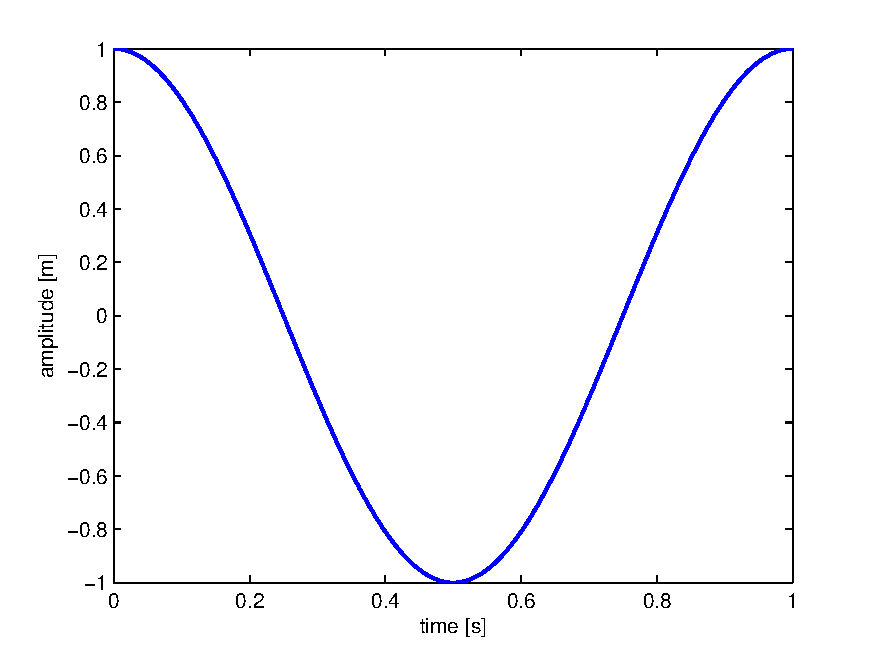
\includegraphics[width=\linewidth]{pic/results}
%	\caption{这是一张图}
%	\label{fig:results}
%\end{figure}

%\begin{equation}\label{key}
%\sum_{n=1}^{\infty} \dfrac{1}{n^2} = \dfrac{\pi^2}{6}.
%\end{equation}


